\section{Introduction}

Diffusion language models (DLMs) are emerging as a competitive text-generation paradigm that combines bidirectional conditioning with parallel, iterative decoding~\cite{nie2025large,bie2025llada2,ye2025dream}. Unlike left-to-right autoregressive (AR) models under causal attention, DLMs use full-sequence bidirectional self-attention within each denoising step, which improves modeling flexibility but changes the inference cost profile: every step must ``see'' the evolving full context rather than only a prefix.

At inference time, this design translates into high generation latency. The dominant cost is bidirectional attention over all query--key pairs---spanning prompt and partially decoded tokens---at \emph{every} denoising step. As total context length $L$ grows, each step incurs $\mathcal{O}(L^2)$ time and memory, which quickly becomes the limiting factor for long-context deployment. Reducing the number of denoising steps is only a partial remedy: DLMs typically need sufficiently many iterations to preserve sample quality, and aggressive step reduction sharply degrades outputs. The practical lever is therefore to improve \emph{per-step} attention efficiency while preserving the denoising trajectory.

Several strategies have been proposed to this end. Semi-autoregressive (block diffusion) methods~\cite{wu2025fastdllm} partition the output into blocks, applying the diffusion process within each block while decoding blocks autoregressively, thereby enabling KV caching across blocks. In a complementary direction, sparse attention---widely adopted in AR models~\cite{jiang2024minference}---identifies important query--key interactions and skips the rest, reducing per-step computation. However, directly transferring AR sparse attention techniques to DLMs is non-trivial due to the fundamentally different attention dynamics of the denoising process.

Existing sparse DLM methods, such as SparseD~\cite{wang2025sparsed}, observe that attention patterns exhibit temporal consistency and therefore compute a sparse attention mask once at an early step and reuse it throughout the remaining denoising trajectory. While this assumption is partially valid, we find that it is insufficient to fully characterize the attention dynamics of DLMs. As shown in Figure~\ref{fig:cross_step}, the attention patterns of DLMs are \emph{locally} consistent across nearby denoising steps but \emph{not globally} stationary. The KL divergence between consecutive steps (Figure~\ref{fig:cross_step_curve}) reveals sharp spikes at certain transition points, indicating abrupt reorganizations of the attention structure as tokens become unmasked and the dependency structure evolves. Consequently, a sparse mask estimated at early steps can become stale: newly important attention links are missed, while computation is wasted on entries that are no longer critical. These observations challenge the one-shot mask reuse paradigm and motivate refreshing the sparse pattern at selected \emph{anchor steps} along the denoising trajectory.

Beyond cross-step dynamics, we identify a second limitation of prior methods: they treat the token as the primary unit of sparsification, implicitly assuming that token importance is consistent across attention heads. Our analysis reveals pronounced \emph{head-wise heterogeneity} in attention concentration. As illustrated in Figure~\ref{fig:attention_heterogeneity}, some heads attend sharply to a small set of key positions, while others distribute attention broadly across the sequence. The cumulative density of attention scores varies markedly: certain heads retain $90\%$ of their attention mass with only $10\%$ of entries, whereas others require close to $50\%$. Applying a uniform sparsity budget across all heads therefore risks over-compressing globally-attending heads while under-compressing locally-focused ones. This observation motivates a \emph{head-adaptive} budget allocation that distributes computation according to each head's functional demands.

\begin{figure}[t]
    \centering
    \begin{subfigure}[b]{0.49\columnwidth}
        \centering
        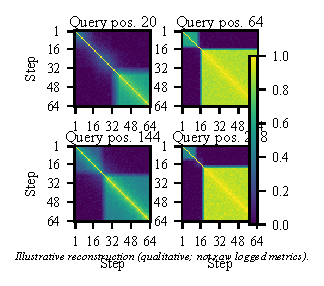
\includegraphics[width=\linewidth]{figures/attention_multi_position.pdf}
        \caption{Cross-step attention similarity for representative query positions.}
        \label{fig:cross_step_heatmap}
    \end{subfigure}
    \hfill
    \begin{subfigure}[b]{0.49\columnwidth}
        \centering
        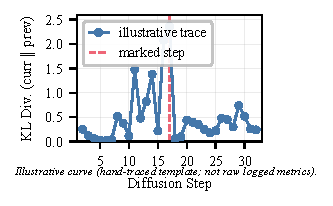
\includegraphics[width=\linewidth]{figures/attention_similarity_curve.pdf}
        \caption{KL divergence between consecutive denoising steps.}
        \label{fig:cross_step_curve}
    \end{subfigure}

    \caption{Attention patterns in DLMs are locally consistent but not globally stationary across denoising steps. (a) Cross-step similarity heatmaps show high similarity within nearby steps but clear discrepancies between distant ones. (b) KL divergence between consecutive steps reveals sharp spikes at transition points, indicating abrupt pattern shifts.}
    \label{fig:cross_step}
\end{figure}

Motivated by these two observations, we propose \textbf{Step-dLLM}, a sparse attention framework tailored for diffusion LLMs. Step-dLLM partitions the denoising trajectory into groups of consecutive steps. The first step in each group serves as an \emph{anchor step} that computes full attention and simultaneously extracts a block-sparse mask; the remaining steps reuse this mask with freshly computed queries, keys, and values, reducing per-step cost from $\mathcal{O}(L^2)$ to $\mathcal{O}(L \cdot k \cdot b)$. The mask is periodically refreshed, bounding its staleness and accommodating the evolving attention structure. Additionally, Step-dLLM allocates a global sparsity budget across heads in proportion to each head's cumulative saliency, allowing concentrated heads to be compressed aggressively while reserving capacity for dispersed yet important ones. Both components are realized through fused Triton kernels---a modified Flash Attention kernel that emits block-level saliency scores as a byproduct, and a block-sparse attention kernel that gathers only the selected key--value blocks---ensuring that the algorithmic gains translate into wall-clock speedups.

In summary, our contributions are as follows:
\begin{itemize}
    \item We present an empirical analysis of sparse attention in diffusion LLMs and identify two key properties: (i) the sparse attention pattern is locally consistent but not globally reusable across denoising steps, and (ii) different attention heads exhibit markedly different concentration behaviors. These findings expose fundamental limitations of one-shot mask reuse and uniform token-level sparsification employed by prior methods.

    \item We propose \textbf{Step-dLLM}, a sparse attention framework for diffusion LLMs that refreshes the sparse mask at selected anchor steps and allocates sparse computation globally across heads according to head-specific saliency, achieving a principled accuracy--efficiency trade-off.

    \item We design fused Triton kernels for both anchor-step mask extraction and non-anchor-step block-sparse attention, and conduct extensive experiments on representative diffusion LLMs, demonstrating that Step-dLLM achieves superior accuracy--efficiency trade-offs compared to prior sparse baselines, especially under high sparsity regimes.
\end{itemize}
